\section{Indirizzi logici}

    Lo \textbf{strato di rete} si occupa della consegna affidabile di pacchetti dati da un nodo mittente ad un nodo destinatario, realizzando un insieme di consegne dirette, ognuna delle quali è gestita dallo strato di collegamento.
    
    Infatti, lo strato di collegamento permette il trasporto di dati (organizzati in frame) fra due nodi immediatamente contigui.
    
    \subsection{Indirizzi IPv4}
    
        Lo strato di rete permette la consegna dei pacchetti tramite l'indirizzamento logico: ogni componente di rete è identificato da un opportuno indirizzo IP. Un indirizzo IPv4 è una sequenza di 32 bit che identifica in modo univoco ed universale un dispositivo connesso ad Internet. Ha una rappresentazione decimale puntata.
        
        \begin{itemize}
            \item
                \textbf{Spazio di indirizzamento IPv$n$.} E' l'insieme dei possibili indirizzi che possono essere utilizzati. Contiene $2^n$ indirizzi.
            
            \item
                \textbf{Spazio di indirizzamento IPv4.} Può contenere al più $2^32$ indirizzi.
        \end{itemize} 
        
        Possiamo suddividere i 32 bit (4 byte) degli indirizzi IP in due parti: prefisso e suffisso. Ogni byte, quantificato fra 0 e 255, è diviso da un punto.
        
        Il prefisso serve per individuare la rete, mentre il suffisso serve per specificare un host sulla medesima rete.
        
        L'indirizzo di rete è importante per il \textit{routing}. Il router filtra le trasmisioni, ammettendole nella rete solo se gli indirizzi di destinazione contengono l'indirizzo di rete del destinatario.
        
        Gli indirizzi IPv4 sono classificati in cinque classi. Per ogni classe, alcuni bit da sinistra vengono riservati, limitando il dominio degli identificativi di rete.
        
        \begin{itemize}
            \item 
                \textbf{Classe A}: indirizzi di unicast. Per organizzazioni grandi.
                
                Hanno un bit iniziale posto a zero. 
                
                7 bit sono dedicati alla rete, mentre i restanti 24 all'host.
            
            \item 
                \textbf{Classe B}: indirizzi di unicast. Per organizzazioni medie.
                
                Hanno due bit iniziali posti a $10$.
                
                14 bit sono dedicati alla rete, mentre i restanti 16 all'host.
                
            \item 
                \textbf{Classe C}: indirizzi di unicast. Per organizzazioni piccole.
                
                Hanno i primi tre bit iniziali posti a $110$.
                
                21 bit sono dedicati alla rete, mentre i restanti 8 all'host.
            
            \item 
                \textbf{Classe D}: indirizzi di multicast. 
                
                Hanno i primi quattro bit posti a $1110$.
                
                28 bit sono dedicati interamente al multicast.
            
            \item 
                \textbf{Classe E}: riservata. 
                
                Hanno i primi 4 bit posti a $1111$. Non è mai stata utilizzata.
                
                28 bit sono riservati.
        \end{itemize}
        
        Ad esempio, un indirizzo di classe C può indirizzare al più $2^21$ reti. Per ciascuna di queste reti, si possono rilevare $2^8$ host.
        
        \begin{center}
            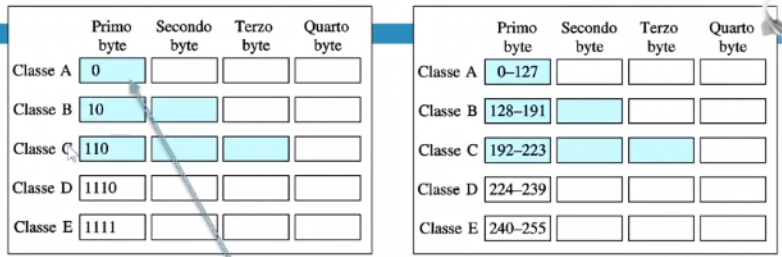
\includegraphics[scale=0.5]{images/Classi-IP.png}
        \end{center}
    
    \subsection{Maschere, subnet e supernet}
    
        La maschera è un metodo per indicare efficientemente la lunghezza dell'indirizzo di rete. In particolare, vengono utilizzate per estrarre rapidamente l'indirizzo di una rete.
        
        \begin{center}
            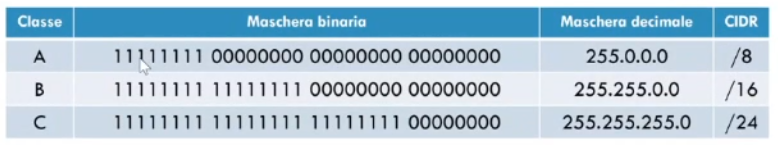
\includegraphics[scale=0.5]{images/Maschera.png}
        \end{center}
        
        Con un'operazione AND bit a bit fra un indirizzo IP e la corrispondete maschera di classe, si ottiene l'indirizzo di rete.
        
        Con un'operazione AND bit a bit fra un indirizzo IP ed il complemento della corrispondente maschera di default, si ottiene l'indirizzo dell'host.
        
        \vspace{3mm}
        
        Il \textbf{subnetting} è utilizzato per dividere un blocco di classe A, B o C, in sottoblocchi di indirizzi consecutivi, ognuno dei quali rappresenta una sottorete. 
        
        L'indirizzo di rete viene \textit{allungato} per avere alcuni bit che servono ad identificare la sottorete all'interno della rete: questo allungamento, in pratica, sovrappone e occupa alcuni bit dell'indirizzo di host per indicare la sottorete.
        
        Gli indirizzi IP hanno una struttura gerarchica. E' detta a 2 livelli se non si usa il subnetting, a 3 livelli se lo si usa.
        
        \vspace{3mm}
        
        Il \textbf{supernetting}, invece, è utilizzato per combinare più blocchi di classe A, B o C in blocchi più grandi.
        
        \vspace{3mm}
        
        Nell'esempio sottostante, la subnet può contenere fino a 254 host distinti (e non 256), poiché gli indirizzi che hanno tutti 0 e tutti 1 (e quindi 256-2) nel campo host sono utilizzati per scopi speciali. Infatti, gli indirizzi con suffisso interamente a 0 identifica la rete, mentre gli indirizzi con suffisso interamente a 1 rappresenta un \textit{indirizzo di broadcast}.
        
        \begin{center}
            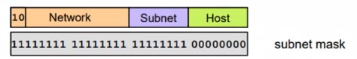
\includegraphics[scale=0.5]{images/Subnet.png}
        \end{center}
        
    \subsection{Indirizzamento senza classi}
    
        L'ndirizzamento con classi e la crescente richiesta, ha portato all'esaurimento degli indirizzi IPv4 disponibili per essere assegnati a nuove reti. L'\textbf{indirizzamento con classi} è ormai obsoleto ed è stato rimpiazzato dall'\textbf{indirizzamento senza classi}.
        
        \vspace{3mm}
        
        Con quest'ultimo schema, non esistono più classi, anche se gli indirizzi vengono comunque assegnati in blocchi. Tali blocchi hanno dimensioni di una qualsiasi potenza di 2 compresa fra $2$ e $2^31$. I blocchi vengono assegnati dal CIDR.
        
        Nell'indirizzamento senza classi, le maschere vengono identificate con la notazione $x.y.z.w/n$, dove $x.y.z.w$ è un qualsiasi indirizzo del blocco, e $/n$ definisce la maschera. $/n$ è chiaramente compreso fra 1 e 31.
        
        Ad esempio, la maschera /23 permette di specificare un blocco di indirizzi IP dotato di $2^9$ indirizzi.
        
        Inoltre, nell'indirizzamento senza classi il prefisso è lungo $n$ bit, e il suffisso $(32-n) bit$.
        
        Per ottenere il primo indirizzo (che identifica la rete o sottorete) si effettua un AND bit a bit con la maschera; per ottenere l'ultimo indirizzo si effettua un OR bit a bit col complemento della maschera.
        
        \begin{center}
            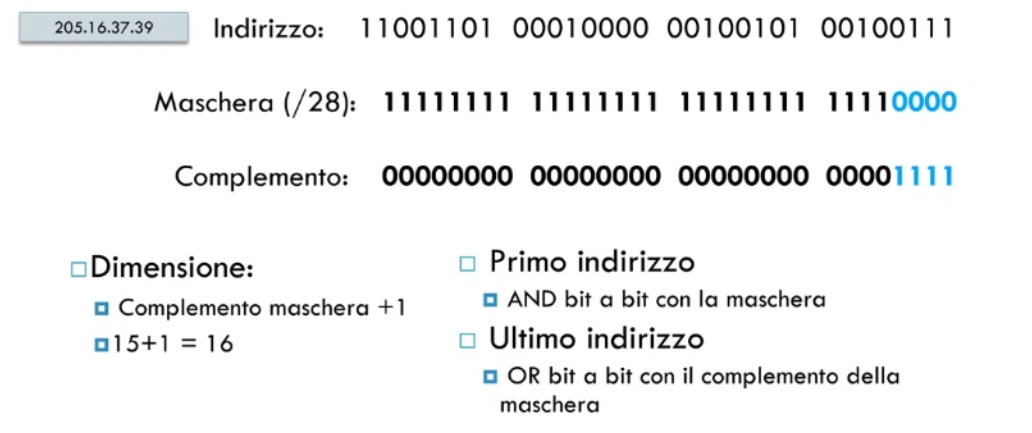
\includegraphics[scale=0.25]{images/EsercizioMaschera.png}
        \end{center}
    
        Gli indirizzi logici vengono assegnati dall'ICANN, che attribuisce grandi blocchi alle ISP. Ogni ISP divide il blocco in sottoblocchi.
        
        \vspace{3mm}
        
        Facciamo un esempio pratico.
        
        Ad un'organizzazione viene assegnato un blocco di indirizzi con indirizzo iniziale $14.24.74.0/24$. Deve assegnare questi indirizzi a tre gruppi di clienti, cioè creare tre sottoblocchi come segue:
        
        \begin{itemize}
            \item Il primo con 10 indirizzi
            \item Il secondo con 60 indirizzi
            \item Il terzo con 120 indirizzi
        \end{itemize}
        
        Osserviamo che in questo blocco si hanno $2^(32-24)=256$ indirizzi. Infatti, $/24$ rappresenta il numero di bit dedicati all'indirizzo di rete. Ne consegue che gli ultimi 8 bit siano dedicati all'indirizzo dell'host.
        
        Il primo indirizzo, ottenuto tramite l'AND bit a bit fra indirizzo e maschera, è $14.24.74.0/24$.
        
        L'ultimo indirizzo, ottenuto tramtie l'OR bit a bit fra indirizzo e complemento della maschera, è $14.24.74.255/24$.
        
        Di questi 256 indirizzi, come creo tre sottoreti da 120, 60 e 10 indirizzi?
        
        \vspace{3mm}
        
        Poiché 120 non è una potenza di 2, si sceglie di allocare 128 indirizzi. La maschera per questa sottorete sarà $n_1 = 32-log_2 128 = 32 - 7 = 25$.
        
        Dato che la maschera è cambiata, possiamo rifare i calcoli (AND bit a bit, OR, etc...) per ottenere il primo e l'ultimo indirizzo di tale sottorete. In particolare, il primo indirizzo della sottorete 1 sarà $14.24.74.0/25$, mentre l'ultimo $14.24.74.127/25$.
        
        Il processo è analogo per le altre due sottoreti. Al termine dell'allocamento, resteranno 48 indirizzi di riserva.
        
        \vspace{3mm}
        
        Infine, definiamo alcuni indirizzi IP particolari.
    
        \begin{itemize}
            \item
                Alcuni blocchi di indirizzi IP sono riservati per uso locale, e cioè non possono essere usati come indirizzi IP pubblici (es. $192.168.0.0)$. Vengono detti \textit{indirizi locali}.
                
            \item
                Gli indirizzi speciali sono $0.0.0.0/8$ (indica questa rete, e questo host) e $127.0.0.0/8$ (indirizzo di \textit{loopback}, per consegnare i pacchetti all'host che li ha spediti).
        \end{itemize}
        
    \subsection{Network Address Translation (NAT)}
    
        Il \textit{NAT} è una tecnica utilizata per ridurre l'impiego di IP pubblici. Internamente, la rete usa indirizzi locali che non sono visibili verso la rete Internet. Un router NAT ha un indirizzo IP pubblico visibile da e verso Internet. 
        
        Tutto il traffico da e verso Internet passa per il router NAT, il quale opera una sorta di traduzione fra indirizzo locale (non pubblico) e indirizzo del router (pubblico). Il router prende l'intestazione e la porta locale della sorgente, sostituendola opportunamente per instradare il reale mittente o destinatario di un pacchetto.
        
        